% !TEX root = ./CM_A-Slides_Annotations.2.2.tex
\providecommand\mainfilename{"./CM_A-Slides_Annotations.tex"}
\providecommand \subfilename{}
\renewcommand   \subfilename{"./CM_A-Slides_Annotations.2.2.tex"}
\documentclass[\mainfilename]{subfiles}

% \tikzset{external/force remake=true} % - remake all

\begin{document}

% \graphicspath{{\subfix{./.build/figures/CM_A-Slides_Annotations.2.2}}}
% \tikzsetexternalprefix{./.build/figures/CM_A-Slides_Annotations.2.2/graphics/}

\mymakesubfile{2}
[CM\,A]
{Caracterização de materiais polímericos} % Subfile Title
{Caracterização de materiais polímericos} % Part Title

\begin{sectionBox}1{Caracterização geral} % S
    
    \begin{center}
        \setlength\tabcolsep{3mm} % width
        % \renewcommand\arraystretch{1.25} % height
        \vspace{1ex}
        \begin{tabular}{l l}
            \toprule
            
                \multicolumn{1}{c}{Critério}
                & \multicolumn{1}{c}{Origem}
            
            \\\midrule
            
                Origem
                & \begin{tabular}{l}
                        \textcolor{Graph21}{Natural}
                    \\  \textcolor{Graph22}{Sintético}
                \end{tabular}
                \\\midrule
                Número de monómeros
                & \begin{tabular}{l}
                        \textcolor{Graph21}{Homopolímero}
                    \\  \textcolor{Graph22}{Copolímero}
                \end{tabular}
                \\\midrule
                Método de preparação
                & \begin{tabular}{l}
                        \textcolor{Graph31}{Polímero de adição}
                    \\  \textcolor{Graph32}{Polímero de condensação}
                    \\  \textcolor{Graph33}{Modificação de outro polímero}
                \end{tabular}
                \\\midrule
                Configuração dos átomos na cadeia
                & \begin{tabular}{l}
                        \textcolor{Graph21}{Sequência cis}
                    \\  \textcolor{Graph22}{Sequência trans}
                \end{tabular}
                \\\midrule
                Taticidade da cadeia polimérica
                & \begin{tabular}{l}
                        \textcolor{Graph31}{Isotático}
                    \\  \textcolor{Graph32}{Sindiotático}
                    \\  \textcolor{Graph33}{Atático}
                \end{tabular} 
                \\\midrule
                Comportamento térmico
                & \begin{tabular}{l}
                        \textcolor{Graph21}{Termoplástico}
                    \\  \textcolor{Graph22}{Termorígido}
                \end{tabular}
                \\\midrule
                Comportamento mecânico
                & \begin{tabular}{l}
                        \textcolor{Graph31}{Borracha ou elastómero}
                    \\  \textcolor{Graph32}{Plástico}
                    \\  \textcolor{Graph33}{Fibra}
                \end{tabular}
            
            \\\bottomrule
        \end{tabular}
        \vspace{2ex}
    \end{center}

    \begin{center}
        \begin{tikzpicture}[sibling distance=10em]
            \node {Polímeros}
                child{node[Graph31]{Naturais}[sibling distance=4em]
                    % child{node{\begin{tabular}{l}
                    %     Proteínas\\Polínucleotidos
                    % \end{tabular}}}
                    child{
                        node{Proteínas,}
                        node[below=1ex]{Polínucleotidos}
                    }
                    child[below=5ex]{node{Polisacarídeos}}
                    child{
                        node{gomas,}
                        node[below=1ex]{resinas}
                    }
                }
                child{node[Graph32]{Elastomeros}}
                child[left=]{node[Graph33]{Sintéticos}[sibling distance=5em]
                    child{node{Termoplásticos}}
                    child[below=2ex]{node{Termoendurecíveis}}
                };
        \end{tikzpicture}
    \end{center}
    
\end{sectionBox}

\begin{sectionBox}2{\color{Graph31}Naturais} % S
    
    Celulose formada por unidades de glicerol.

    \begin{center}
        \begin{tikzpicture}[sibling distance=10em]
            \node{Naturais}
            % child{node{\begin{tabular}{l}
            %     Proteínas\\Polínucleotidos
            % \end{tabular}}}
            child{
                node[GraphA11]{Proteínas,}
                node[GraphA13][below=1ex]{Polínucleotidos}
            }
            child{node[GraphA15]{Polisacarídeos}}
            child{
                node[GraphA17]{gomas,}
                node[GraphA19][below=1ex]{resinas}
            };
        \end{tikzpicture}
    \end{center}

    \paragraph*{\color{GraphA11}Proteínas:} 
    Sequencias de \emph{aminoácidos} ligados por \emph{ligações peptidicas}
    \paragraph*{\color{GraphA13}Polinucleótido:}
    Sequencia de \emph{nucleótidos}, exemplo: \emph{DNA}
    \paragraph*{\color{GraphA15}Polissacarídeos:}
    \emph{Monossacarídeos} ligados por por \emph{ligações glicosídicas}

    \begin{sectionBox}*3{Biopolímeros} % S
        
        \begin{center}
            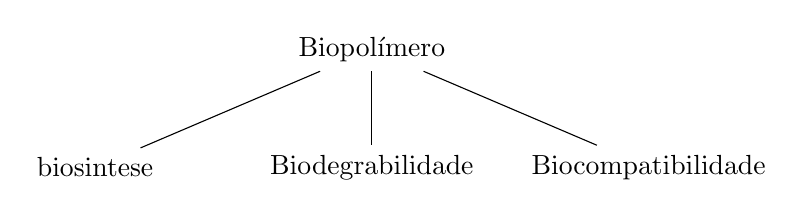
\begin{tikzpicture}[sibling distance=10em]
                \node{Biopolímero}
                child{node{biosintese}}
                child{node{Biodegrabilidade}}
                child{node{Biocompatibilidade}};
            \end{tikzpicture}
        \end{center}
        
        A maioria são polímeros naturais
        \paragraph*{Poliésteres produzidos por bactérias:}
        \begin{itemize}
            \begin{multicols}{2}
                \item polihidroxialcanoatos,
                \item PHB (polihidroxibutirato),
                \item Copoli(HB/HV),
                \item Copoli(hidroxibutirat/valerato)
                \item Com propriedades físicas semelhantes ao PP
            \end{multicols}
        \end{itemize}
        \paragraph*{Proteínas}
        \begin{itemize}
            \begin{multicols}{2}
                \item Seda
                \item lã
            \end{multicols}
        \end{itemize}
        \paragraph*{Produzidos industrialmente}
        \begin{itemize}
            \begin{multicols}{2}
                \item Poli(ácido láctico)
                \item Poliglicosido
            \end{multicols}
        \end{itemize}

    \end{sectionBox}
    % \paragraph*{\color{GraphA15}B}
    
\end{sectionBox}

\begin{sectionBox}2{\color{Graph32}Elastomeros} % S
    
    Capacidade de deformar sobre tensão e retornar a sua forma original quando a tensão é removida
    
\end{sectionBox}

\begin{sectionBox}2{\color{Graph33}Sintéticos (Plásticos)} % S
    
    Em geral produtos derivados do petróleo, tamanho e composição quimica podem ser manipulados para manifestar todos os tipos de propriedades

    \begin{center}
        \begin{tikzpicture}[sibling distance=10em]
            \node{Sintéticos}
            child{node[Graph21]{Termoplásticos}}
            child{node[Graph22]{Termodurecíveis}};
        \end{tikzpicture}
    \end{center}
    \paragraph*{\color{Graph21}Termoplásticos:}
    Aquecidos até á sua temperatura de fusão, apóarrefecimento retomam as suas características
iniciais. São polímeros lineares ou ramificados.
\end{sectionBox}

\end{document}